\subsubsection{UC3 - Inserimento richiesta in linguaggio naturale}\label{UC3}

\begin{figure}[H]
  \centering
  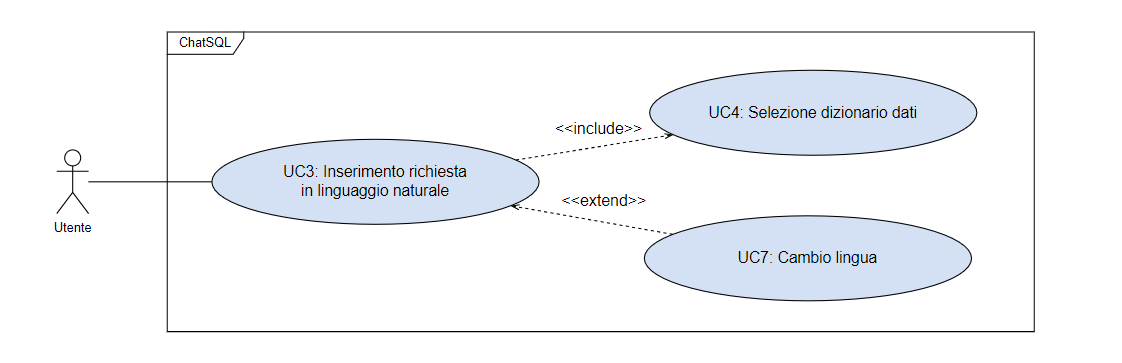
\includegraphics[width=0.90\textwidth]{assets/uc3.png}
  \caption{UC3}
\end{figure}

\paragraph*{Descrizione}
L’Utente desidera inserire una richiesta in qualsiasi linguaggio naturale al fine di ottenere il \glossario{prompt} che selezioni la parte del \glossario{dizionario dati} più inerente alla richiesta. 

\paragraph*{Attori principali}
Utente

\paragraph*{Precondizioni}
\begin{itemize}
  \item L'applicazione è stata avviata con successo;
  \item L’Utente ha in precedenza selezionato un \glossario{dizionario dati} (\hyperref[UC4]{UC4}); 
  \item L'Utente seleziona la lingua di inserimento, se non selezionata viene utilizzato l'italiano di default (\hyperref[UC7]{UC7}).
\end{itemize}

\paragraph*{Postcondizioni}
\begin{itemize}
  \item L’Utente ha scritto nell’apposito campo di testo un'interrogazione in linguaggio naturale.
\end{itemize}

\paragraph*{Scenario principale}
\begin{enumerate}
  \item L’Utente scrive un'interrogazione nell’apposito box su cui poi il sistema potrà produrre un \glossario{prompt} in seguito.
\end{enumerate}

\paragraph*{Inclusioni}
\begin{itemize}
  \item Selezione \glossario{dizionario dati} (\hyperref[UC4]{UC4});
\end{itemize}

\paragraph*{Estensioni}
\begin{itemize}
  \item Cambio lingua (\hyperref[UC7]{UC7});
\end{itemize}